\section{Systemmodelle}

\subsection{Objektmodelle}

\begin{figure}[H]
\centering
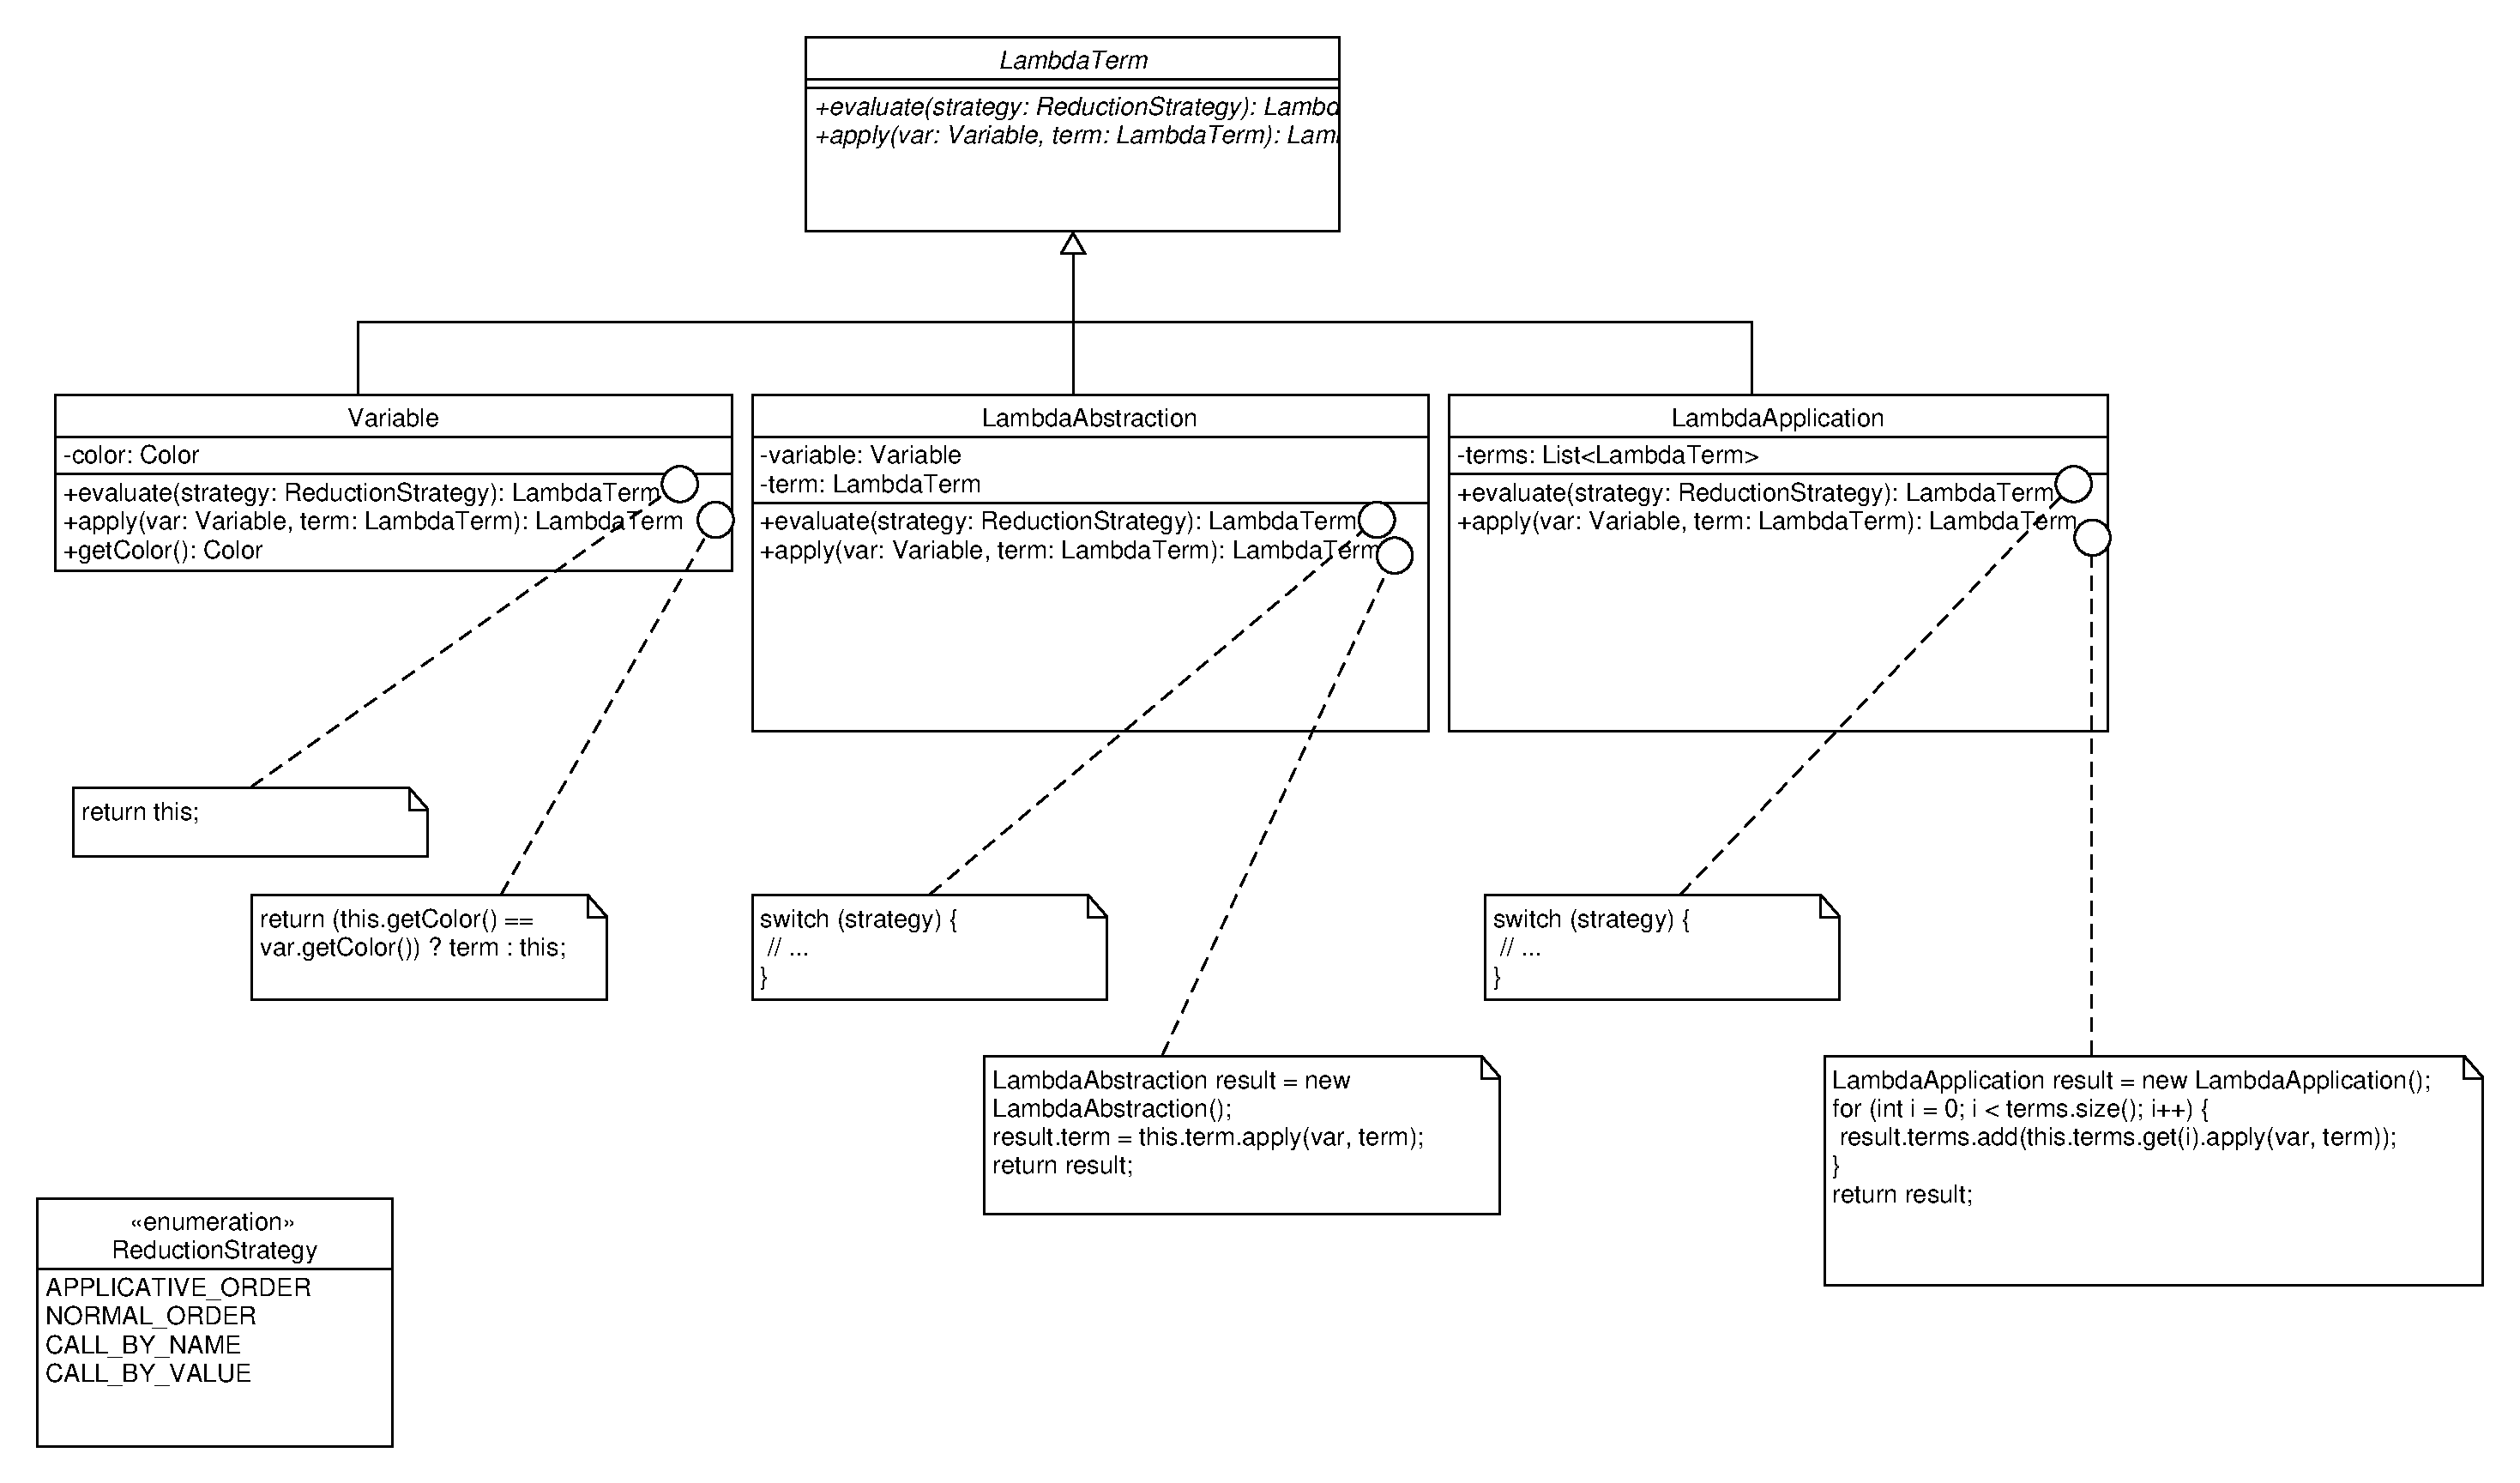
\includegraphics[scale=0.5]{../system_models/object_models/lambda_calculus.pdf}
\caption{UML Klassendiagramm zum Lambda-Kalkül}
\end{figure}

\subsection{Dynamische Modelle}

\begin{figure}[H]
\centering
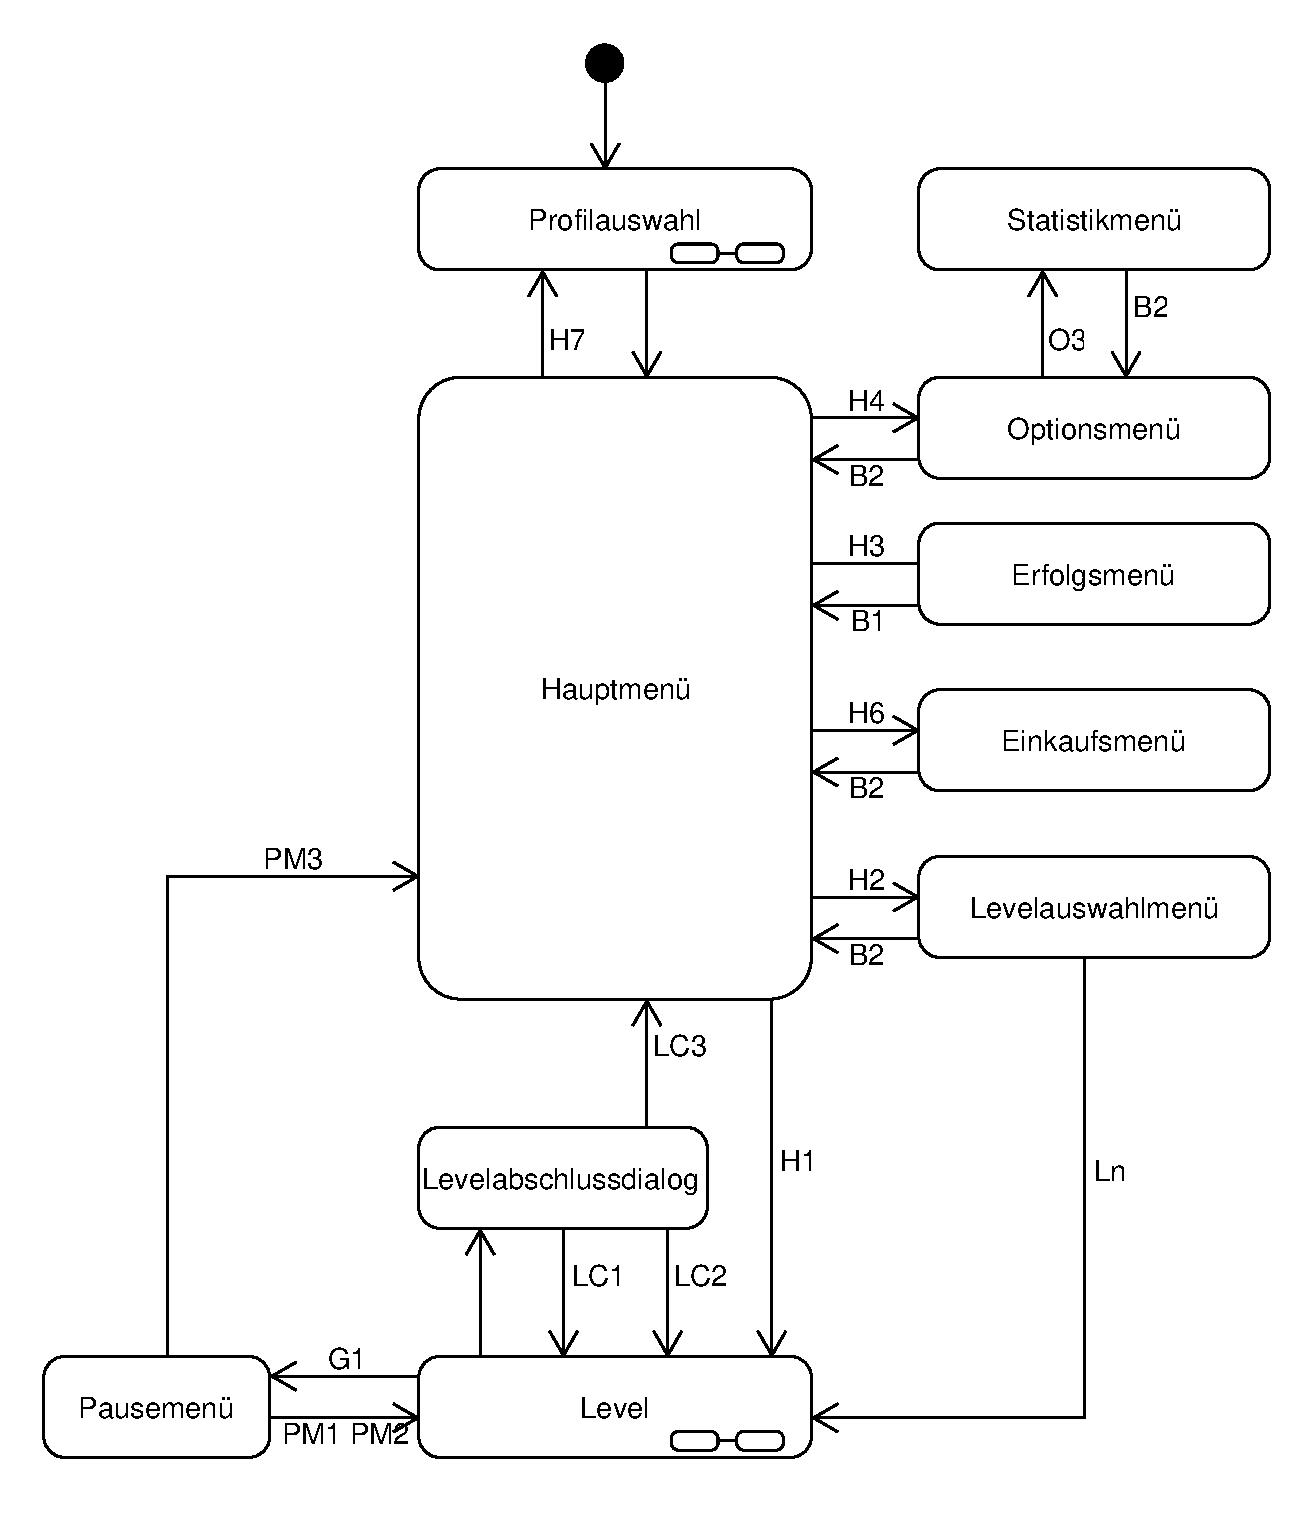
\includegraphics[scale=0.65]{../system_models/dynamic_models/menu_state_machine.pdf}
\caption{Zustandsautomat zur Menübedienung}
\end{figure}

\begin{figure}[H]
\centering
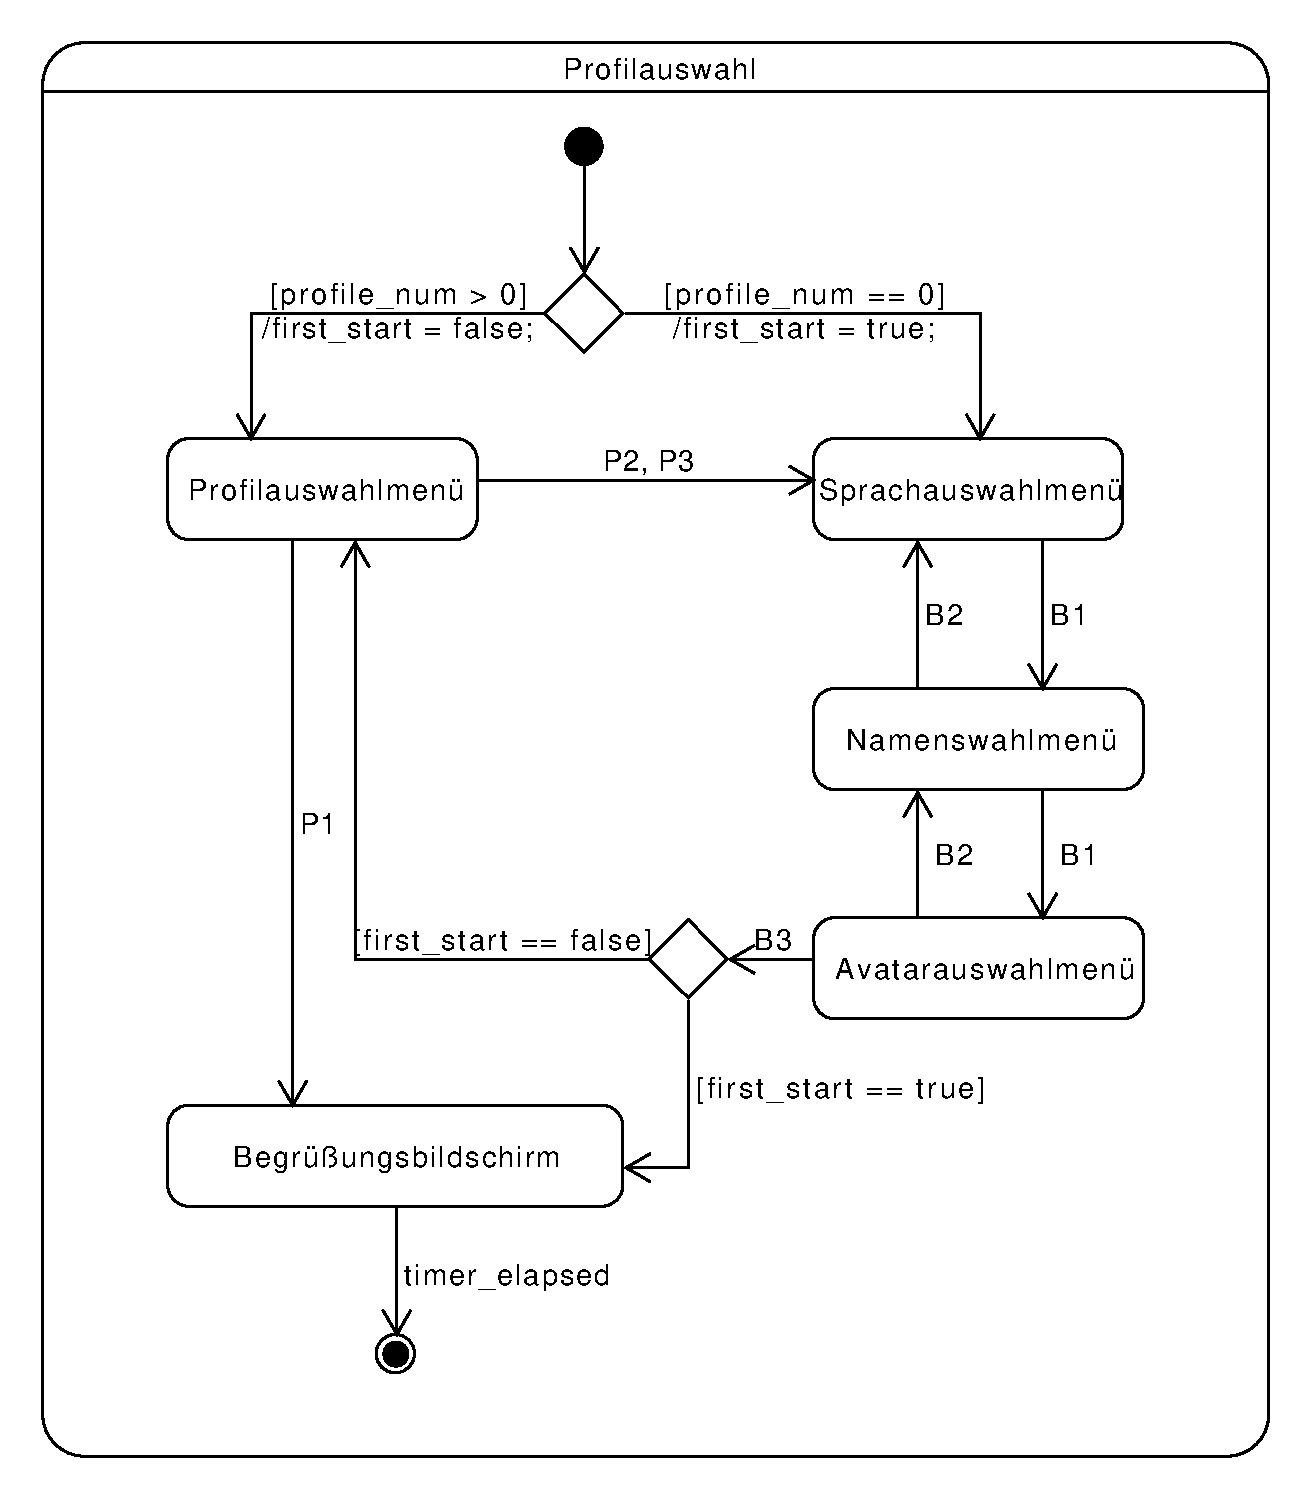
\includegraphics[scale=0.6]{../system_models/dynamic_models/profile_selection_state_machine.pdf}
\caption{Zustandsautomat zur Profilerstellung/-editierung/-auswahl}
\end{figure}

\begin{figure}[H]
\centering
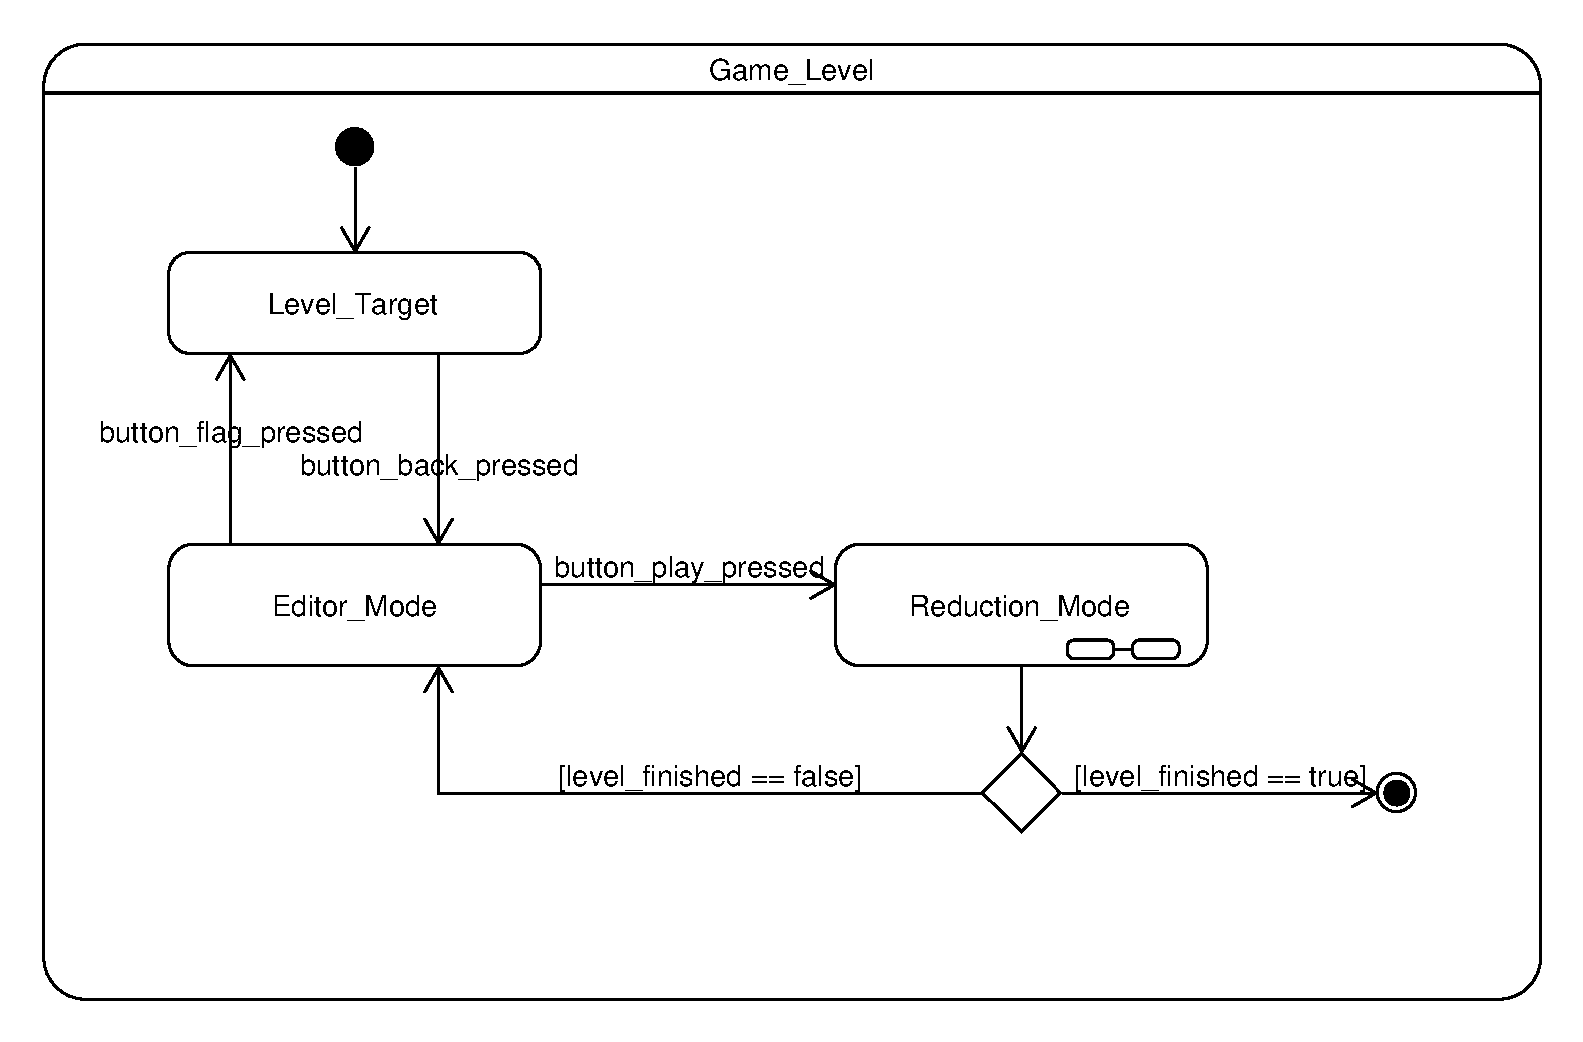
\includegraphics[scale=0.65]{../system_models/dynamic_models/game_level_state_machine.pdf}
\caption{Zustandsautomat zum Ablauf eines Levels}
\end{figure}

\begin{figure}[H]
\centering
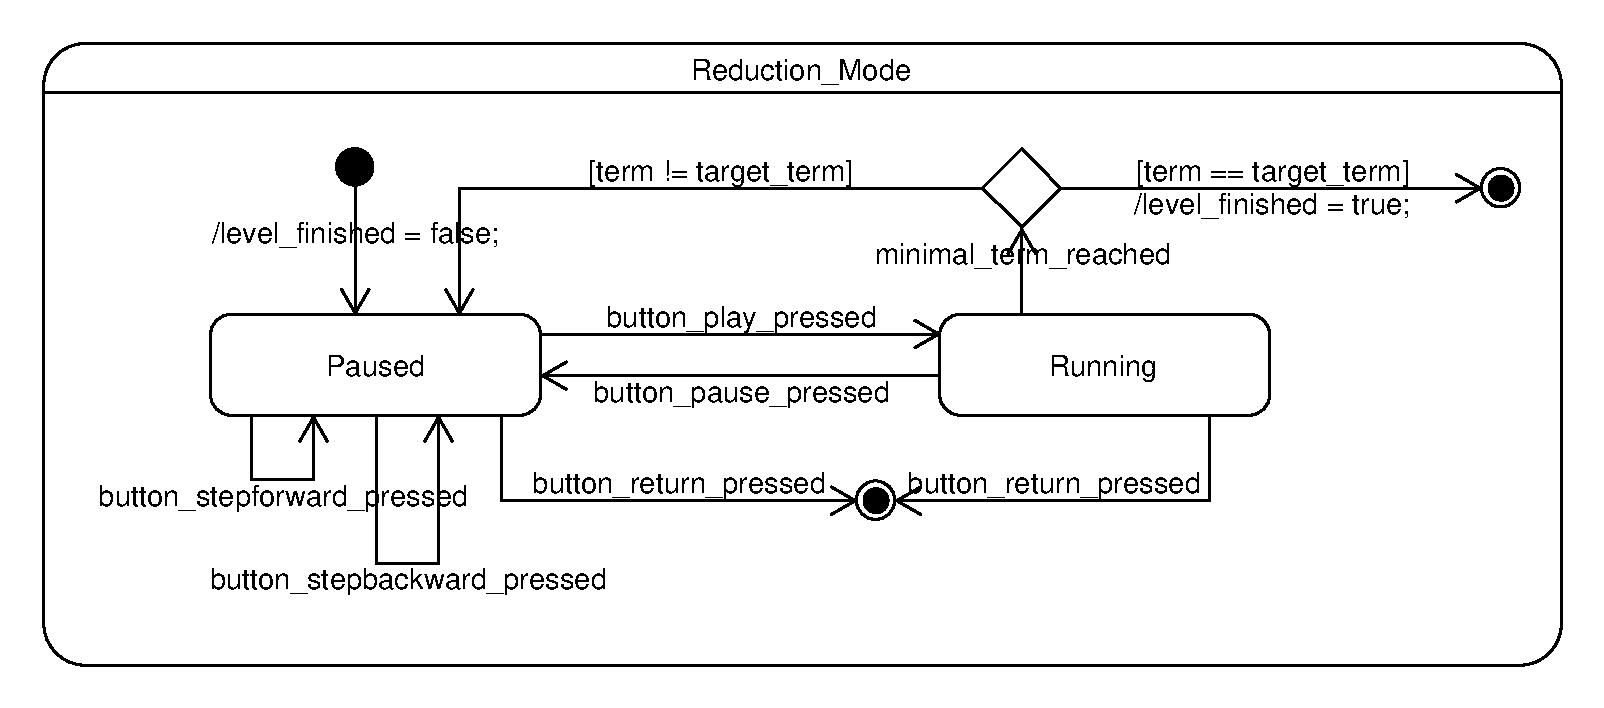
\includegraphics[scale=0.67]{../system_models/dynamic_models/reduction_mode_state_machine.pdf}
\caption{Zustandsautomat zur Funktion des Reduktionsmodus}
\end{figure}

\subsection{Benutzerschnittstelle}
\label{gui_section}

% ---------------------- Sprachauswahlmenü ----------------------

\begin{figure}[H]
\centering
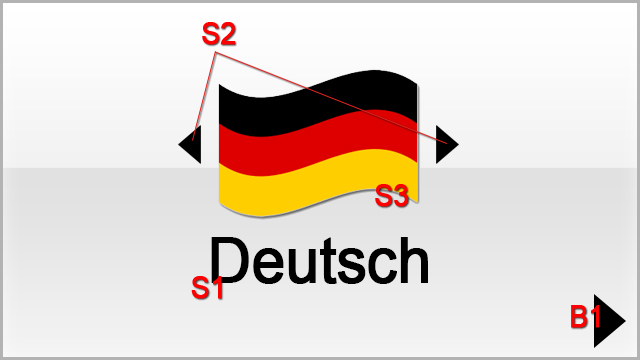
\includegraphics[scale=0.55]{../gui/_jpeg_numeration/registration1.jpg}
\caption{Sprachauswahlmenü}
\label{fig:Sprachauswahlmenu}
\end{figure}
\begin{description*}
\item[S1] Sprachen-Label: Zeigt aktuell ausgewählte Sprache an
\item[S2] Sprachenauswahl-Buttons: Zum Wechseln der Sprache
\item[S3] Flaggen-Image: Zeigt aktuell ausgewählte Sprache an
\item[B1] Weiter-Button: Zum Wechsel in das Namenswahlmenü $($Abb. \ref{fig:Namenswahlmenu}$)$
\end{description*}

% ---------------------- Namenswahlmenu ----------------------

\begin{figure}[H]
\centering
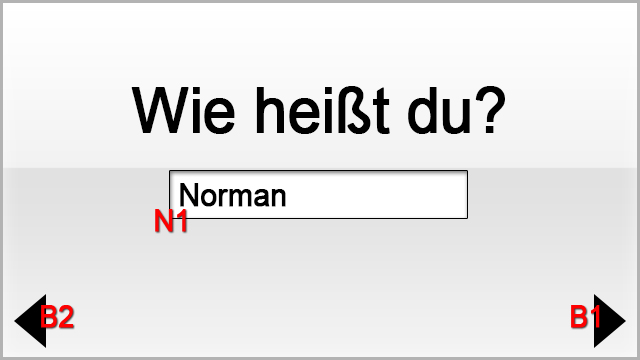
\includegraphics[scale=0.55]{../gui/_jpeg_numeration/registration2.jpg}
\caption{Namenswahlmenü}
\label{fig:Namenswahlmenu}
\end{figure}
\begin{description*}
\item[N1] Namenseingabe-Textbox: Zur Eingabe des Namens
\item[B2] Zurück-Button: Zum Wechsel in das Sprachauswahlmenü $($Abb. \ref{fig:Sprachauswahlmenu}$)$
\item[B1] Weiter-Button: Zum Wechsel in das Avatarauswahlmenü $($Abb. \ref{fig:Avatarauswahlmenu}$)$
\end{description*}

% ---------------------- Avatarauswahlmenü ----------------------

\begin{figure}[H]
\centering
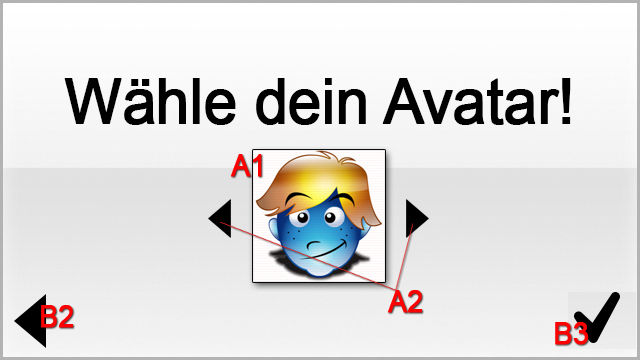
\includegraphics[scale=0.55]{../gui/_jpeg_numeration/registration3.jpg}
\caption{Avatarauswahlmenü}
\label{fig:Avatarauswahlmenu}
\end{figure}
\begin{description*}
\item[A1] Avatar-Image: Zeigt aktuell ausgewählten Avatar an
\item[A2] Avatarauswahl-Buttons: Zum Wechseln des Avatars
\item[B2] Zurück-Button: Zum Wechsel in das Namenswahlmenü $($Abb. \ref{fig:Namenswahlmenu}$)$
\item[B3] Bestätigungs-Button: Zum Beenden der Profileditierung
\end{description*}

% ---------------------- Profilauswahlmenu ----------------------

\begin{figure}[H]
\centering
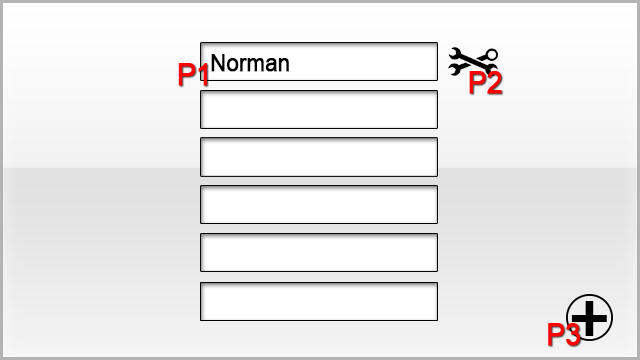
\includegraphics[scale=0.55]{../gui/_jpeg_numeration/choose_profile.jpg}
\caption{Profilauswahlmenü}
\label{fig:Profilauswahlmenu}
\end{figure}
\begin{description*}
\item[P1] Name-Button: Zum Einloggen eines Profils
\item[P2] Konfigurations-Button: Zum Editieren und Löschen eines Profils
\item[P3] Hinzufügen-Button: Zum Hinzufügen eines Profils
\end{description*}

% ---------------------- BegrüssŸungsbildschirm ----------------------

\begin{figure}[H]
\centering
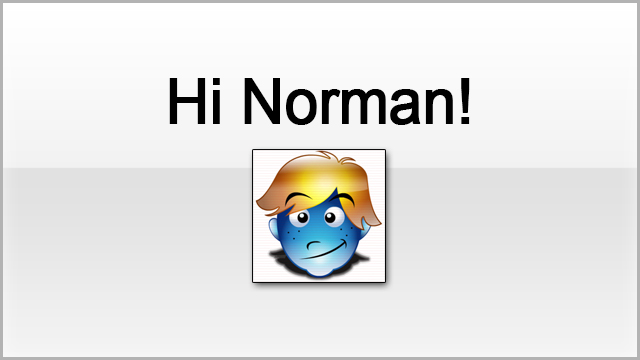
\includegraphics[scale=0.55]{../gui/_jpeg_numeration/welcome.jpg}
\caption{Begrüßungsbildschirm}
\label{fig:Begrussungsbildschirm}
\end{figure}
%\begin{description*}
%\end{description*}

% ---------------------- Hauptmenü ----------------------

\begin{figure}[H]
\centering
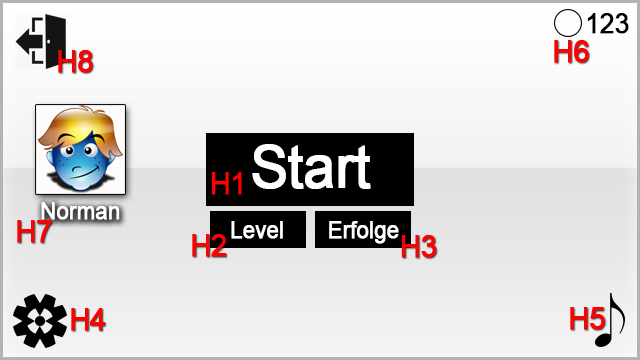
\includegraphics[scale=0.55]{../gui/_jpeg_numeration/main_manu.jpg}
\caption{Hauptmenü}
\label{fig:Hauptmenu}
\end{figure}
\begin{description*}
\item[H1] Start-Button: Zum Starten des zuletzt freigeschalteten Levels
\item[H2] Level-Button: Zum Wechsel in das Levelauswahlmenü $($Abb. \ref{fig:Levelauswahlmenu}$)$
\item[H3] Erfolge-Button: Zum Wechsel in das Erfolgsmenü $($Abb. \ref{fig:Erfolgsmenu}$)$
\item[H4] Optionen-Button: Zum Wechsel in das Optionsmenü $($Abb. \ref{fig:Optionsmenu}$)$
\item[H5] Stumm-Checkbox: Zum An-/Ausschalten der Hintergrundmusik
\item[H6] Einkaufs-Button: Zum Wechsel in das Einkaufsmenü $($Abb. \ref{fig:Einkaufsmenu}$)$
\item[H7] Logout-Button: Zum Wechsel in das Profilauswahlmenü $($Abb. \ref{fig:Profilauswahlmenu}$)$
\end{description*}

% ---------------------- Optionsmenü ----------------------

\begin{figure}[H]
\centering
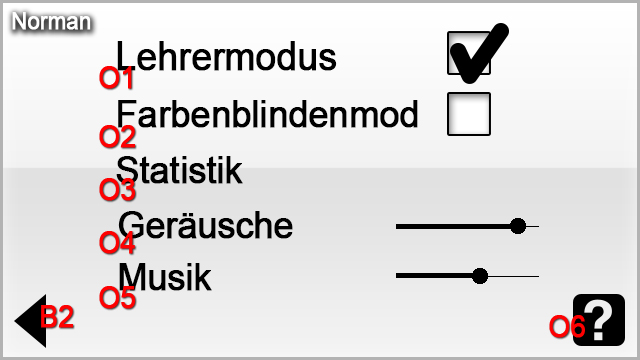
\includegraphics[scale=0.55]{../gui/_jpeg_numeration/settings.jpg}
\caption{Optionsmenü}
\label{fig:Optionsmenu}
\end{figure}
\begin{description*}
\item[O1] Lehrermodus-Checkbox: Zum Ein-/Ausschalten des Lehrermodus
\item[O2] Farbenblindenmodus-Checkbox: Zum Ein-/Ausschalten des Farbenblindenmodus
\item[O3] Statistik-Button: Zum Wechsel in das Statistikmenü $($Abb. \ref{fig:Statistikmenu}$)$
\item[O4] Geräusche-Slider: Zum Einstellen der Geräuschlautstärke
\item[O5] Musik-Slider: Zum Einstellen der Hintergrundmusiklautstärke
\item[O6] Hilfe-Button: Gibt Hilfe zum Optionsmenü
\item[B2] Zurück-Button: Zum Wechsel in das Hauptmenü $($Abb. \ref{fig:Hauptmenu}$)$
\end{description*}

% ---------------------- Statistikmenü ----------------------

\begin{figure}[H]
\centering
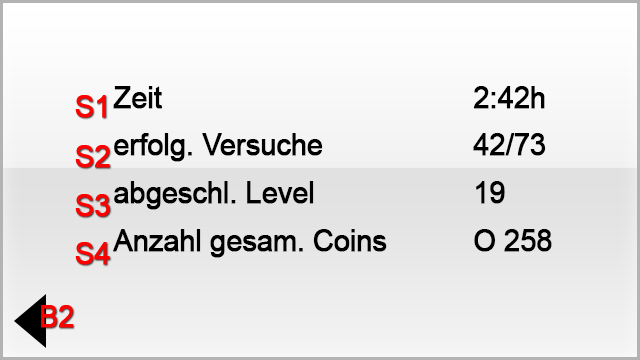
\includegraphics[scale=0.55]{../gui/_jpeg_numeration/stat.jpg}
\caption{Statistikmenü}
\label{fig:Statistikmenu}
\end{figure}
\begin{description*}
\item[Sn] Statistik-Label: Zeigt ein Statistik-Datum an
\item[B2] Zurück-Button: Zum Wechsel in das Optionsmenü $($Abb. \ref{fig:Optionsmenu}$)$
\end{description*}

% ---------------------- Editormodus ----------------------

\begin{figure}[H]
\centering
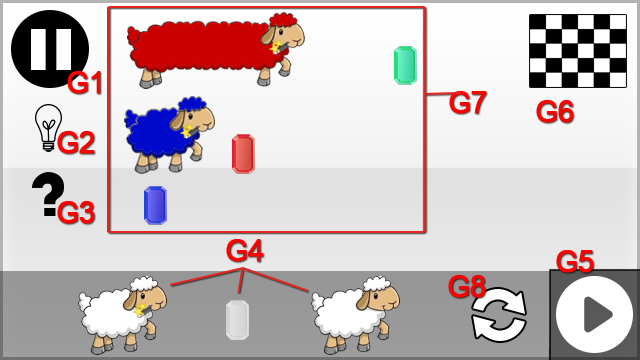
\includegraphics[scale=0.55]{../gui/_jpeg_numeration/game.jpg}
\caption{Editormodus}
\label{fig:Editormodus}
\end{figure}
\begin{description*}
\item[G1] Pause-Button: Zum Anzeigen des Pause-Dialogs $($Abb. \ref{fig:Editormodus_Paused}$)$
\item[G2] Hinweis-Button: Zum Anzeigen von Tipps zum Level
\item[G3] Hilfe-Button: Gibt Hilfe zum Editormodus
\item[G4] Drag$\&$Drop-Elemente: Zum Erstellen eines Terms
\item[G5] Reduktions-Button: Zum Wechsel in den Reduktionsmodus $($Abb. \ref{fig:Reduktionsmodus}$)$ mit aktuellem Term und Reduktionsstrategie
\item[G6] Levelziel-Button: Zum Anzeigen des Levelziels
\item[G7] Term-View: Zeigt aktuellen Term an
\item[G8] Reduktionsstrategie-Button: Zur Auswahl der Reduktionsstrategie
\end{description*}

% ---------------------- Pause-Dialog ----------------------

\begin{figure}[H]
\centering
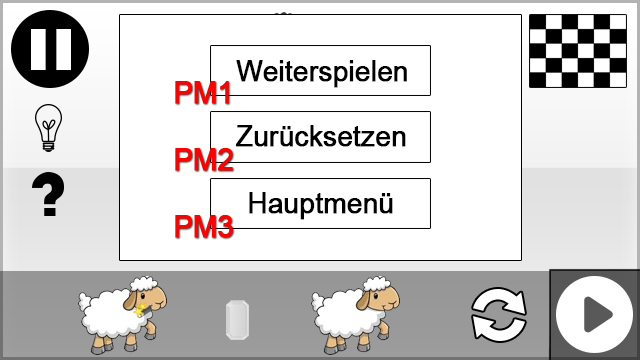
\includegraphics[scale=0.55]{../gui/_jpeg_numeration/game_paused.jpg}
\caption{Pause-Dialog}
\label{fig:Editormodus_Paused}
\end{figure}
\begin{description*}
\item[PM1] Weiterspielen-Button: Schließt den Pause-Dialog
\item[PM2] Zurücksetzen-Button: Setzt den Term auf auf die Levelvorgabe zurück
\item[PM3] Hauptmenü-Button: Beendet das Level und wechselt zum Hauptmenü
\end{description*}

% ------------ Editormodus mit aktiviertem Lehrermodus ---------------

\begin{figure}[H]
\centering
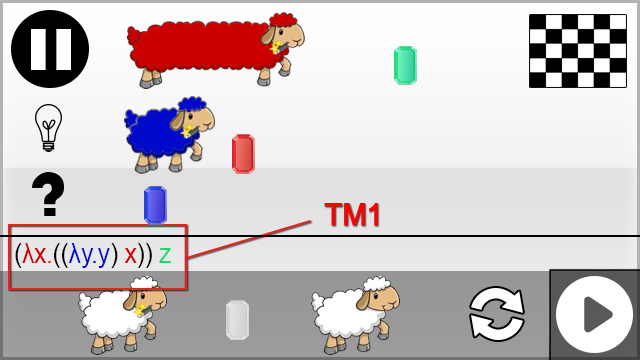
\includegraphics[scale=0.55]{../gui/_jpeg_numeration/game_teachermode.jpg}
\caption{Editormodus mit aktiviertem Lehrermodus}
\label{fig:Editormodus_TM}
\end{figure}
\begin{description*}
\item[TM1] Lambdaterm-Label: Zeigt aktuellen Term in Lambdakalkül-Schreibeweise an
\end{description*}

% ---------------------- Reduktionsmodus ----------------------

\begin{figure}[H]
\centering
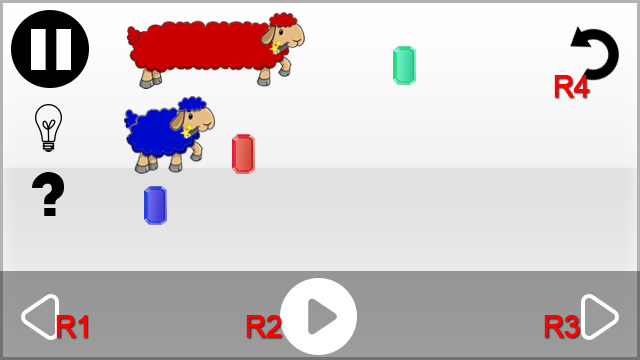
\includegraphics[scale=0.55]{../gui/_jpeg_numeration/game_play_started.jpg}
\caption{Reduktionsmodus}
\label{fig:Reduktionsmodus}
\end{figure}
\begin{description*}
\item[R1] Schritt-Rückwärts-Button: Macht den letzten Reduktionsschritt rückgängig
\item[R2] Abspiel-Button: Startet das automatische Reduzieren
\item[R3] Schritt-Vorwärts-Button: Führt einen Reduktionsschritt aus
\item[R4] Zurück-Button: Wechselt zurück in den Editormodus $($Abb. \ref{fig:Editormodus}$)$
\end{description*}

% ---------------------- Levelabschluss ----------------------

\begin{figure}[H]
\centering
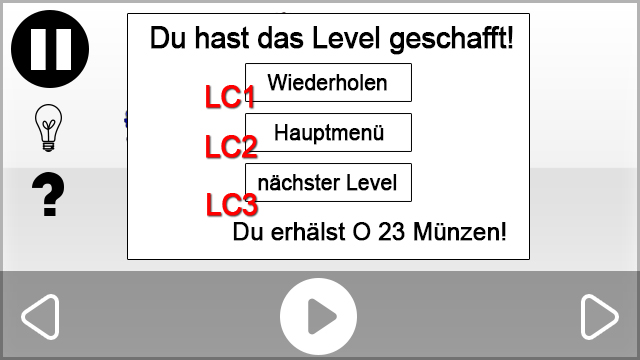
\includegraphics[scale=0.55]{../gui/_jpeg_numeration/game_completed.jpg}
\caption{Levelabschluss-Dialog}
\label{fig:Reduktionsmodus_Levelabschluss}
\end{figure}
\begin{description*}
\item[LC1] Wiederholen-Button: Startet dasselbe Level erneut
\item[LC2] Hauptmenü-Button: Wechselt in das Hauptmenü $($Abb. \ref{fig:Hauptmenu}$)$
\item[LC3] Nächster-Level-Button: Startet das nächste Level
\end{description*}

% ---------------------- Freier Editor ----------------------

%\begin{figure}[H]
%\centering
%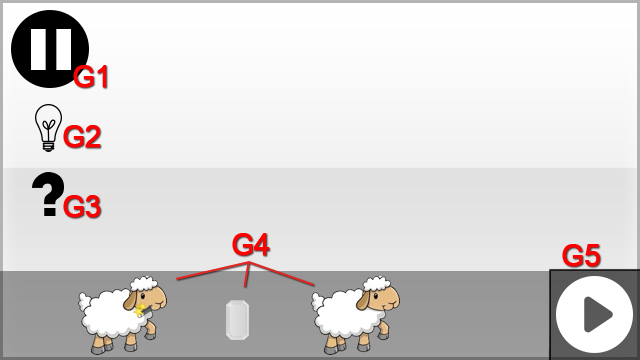
\includegraphics[scale=0.55]{../gui/_jpeg_numeration/game_freemode.jpg}
%\caption{Freier Editor}
%\label{fig:Freier Editor}
%\end{figure}
%\begin{description*}
%\end{description*}

% ---------------------- Erfolgsmenü ----------------------

\begin{figure}[H]
\centering
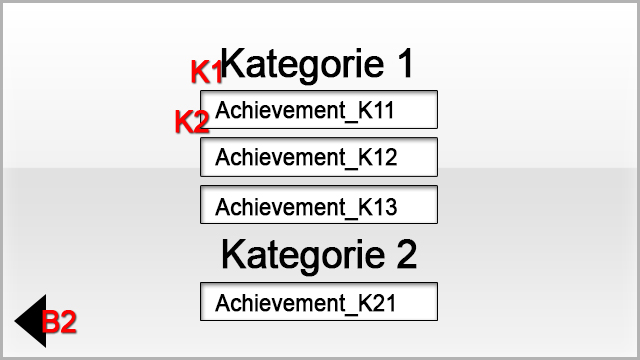
\includegraphics[scale=0.55]{../gui/_jpeg_numeration/achievements.jpg}
\caption{Erfolgsmenü}
\label{fig:Erfolgsmenu}
\end{figure}
\begin{description*}
\item[K1] Kategorie-Label: Überschrift für eine Menge von Erfolgen
\item[K2] Achievement-Label: Beschreibung eines einzelnen Erfolges
\item[B1] Zurück-Button: Wechselt in das Hauptmenü $($Abb. \ref{fig:Hauptmenu}$)$
\end{description*}

% ---------------------- Levelauswahlmenü ----------------------

\begin{figure}[H]
\centering
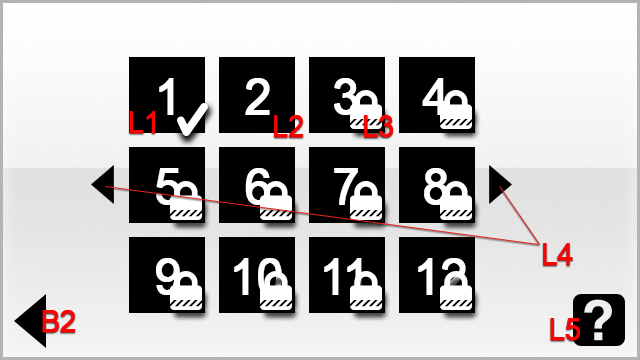
\includegraphics[scale=0.55]{../gui/_jpeg_numeration/level.jpg}
\caption{Levelauswahlmenü}
\label{fig:Levelauswahlmenu}
\end{figure}
\begin{description*}
\item[Ln] Levelstart-Button: Startet das gewählte Level
\item[L1] Levelstart-Button mit Haken: Freigeschaltetes Level, welches abgeschlossen wurde
\item[L2] Levelstart-Button ohne Haken: Freigeschaltetes Level, welches nicht abgeschlossen wurde
\item[L3] Levelstart-Button mit Schloss: Nicht freigeschaltetes Level
\item[L4] Seitenauswahl-Button: Wechselt zwischen Seiten mit Leveln
\item[L5] Hilfe-Button: Gibt Hilfe zum Levelauswahlmenü
\item[B2] Zurück-Button: Wechselt in das Hauptmenü $($Abb. \ref{fig:Hauptmenu}$)$
\end{description*}

% ---------------------- Einkaufsmenü ----------------------

\begin{figure}[H]
\centering
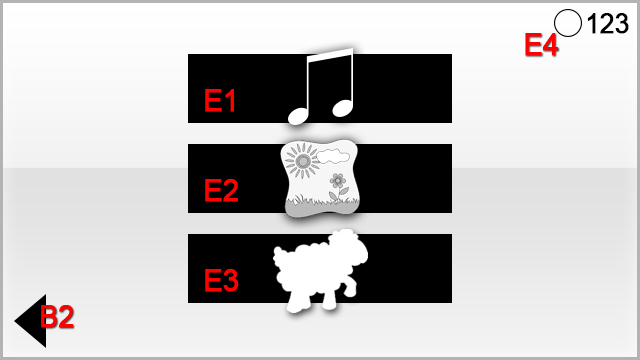
\includegraphics[scale=0.55]{../gui/_jpeg_numeration/shop.jpg}
\caption{Einkaufsmenü}
\label{fig:Einkaufsmenu}
\end{figure}
\begin{description*}
\item[E1] Musik-Dropdownmenü: Zeigt kaufbare Hintergrundmusikstücke an
\item[E2] Hintergrund-Dropdownmenü: Zeigt kaufbare Hintergrundbilder an
\item[E3] Texturen-Dropdownmenü: Zeigt kaufbare Texturbilder an
\item[E4] Münzen-Label: Zeigt aktuelle Anzahl von Münzen an
\item[B2] Zurück-Button: Wechselt in das Hauptmenü $($Abb. \ref{fig:Hauptmenu}$)$
\end{description*}

% ---------- Einkaufsmenü mit gess¶ffnetem Musik-Dropdownmenü ----------

\begin{figure}[H]
\centering
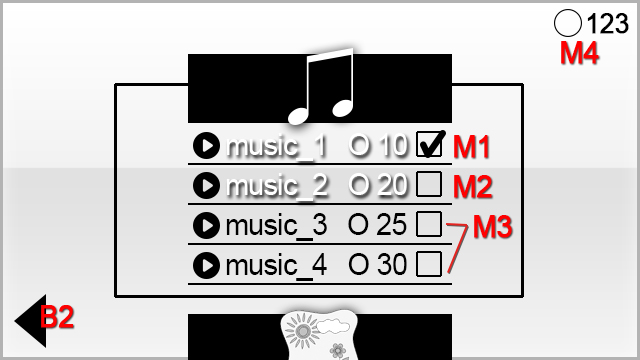
\includegraphics[scale=0.55]{../gui/_jpeg_numeration/shop_popup.jpg}
\caption{Einkaufsmenü mit geöffnetem Musik-Dropdownmenü}
\label{fig:Einkaufsmenu_Dropdown}
\end{figure}
\begin{description*}
\item[Mn] Shopelement-Button: Gibt Informationen zum kaufbaren Objekt, dient zum Kauf und zur Aktivierung
\item[M1] Weisser Showelement-Button mit Haken: Zeigt an, dass dieses Element erworben und aktiviert ist
\item[M2] Weisser Shopelement-Button ohne Haken: Zeigt an, dass dieses Element erworben, aber nicht aktiviert ist
\item[M3] Schwarzer Showelement-Button: Zeigt an, dass dieses Element erworben werden kann
\end{description*}
